\documentclass{article}
\usepackage{amsmath,amssymb}
\usepackage[numbers]{natbib}
\usepackage{geometry}
 \geometry{
 a4paper,
 total={170mm,257mm},
 left=30mm,
 top=30mm,
 right=30mm,
 bottom=30mm
 }
\usepackage{graphicx}
\usepackage{multirow}
\usepackage{siunitx}
\usepackage{booktabs}
\usepackage{gensymb}
\usepackage{float}
\usepackage{tikz}
\usetikzlibrary{chains}
\graphicspath{ {../tmp/} }

\setlength{\parskip}{1em}

\title{Reinforcement Learning Assignment-1}
\begin{document}
\author{Utkarsh Prakash \\ \normalsize 180030042}
\maketitle
\begin{enumerate}
    \item Histogram obtained after sampling $N=100$ samples:
        \begin{figure}[H]
            \begin{center}
            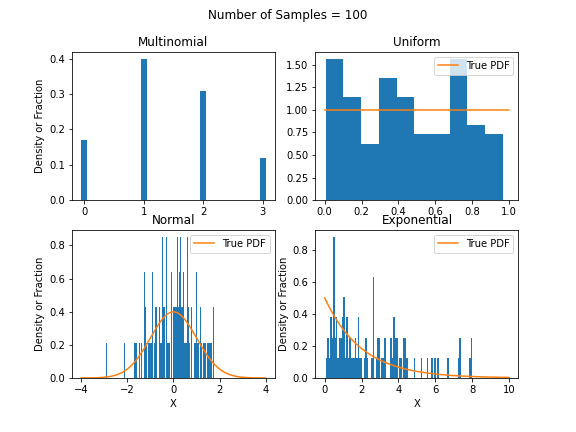
\includegraphics[width=10cm]{Q1_100.png}
            \end{center}
            \caption{Histogram obtained after sampling $N=100$ samples.}
        \end{figure}
        Here, since the number of samples is less hence we see a lot deviation between the plotted histogram and the true PDF.\par
	
	    \noindent %The next paragraph is not indented
        Histogram obtained after sampling $N=1000$ samples:
        \begin{figure}[H]
            \begin{center}
            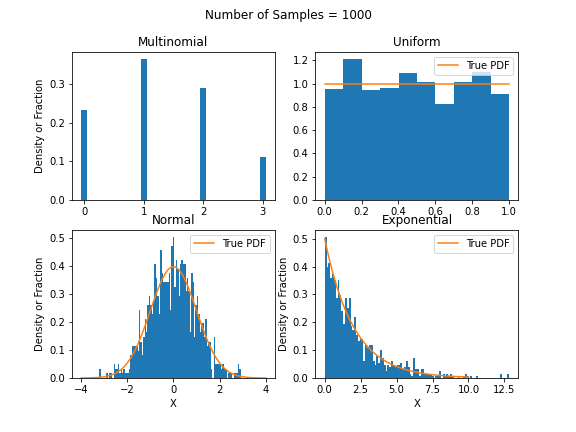
\includegraphics[width=10cm]{Q1_1000.png}
            \end{center}
            \caption{Histogram obtained after sampling $N=1000$ samples.}
        \end{figure}

        Histogram obtained after sampling $N=10000$ samples:
        \begin{figure}[H]
            \begin{center}
            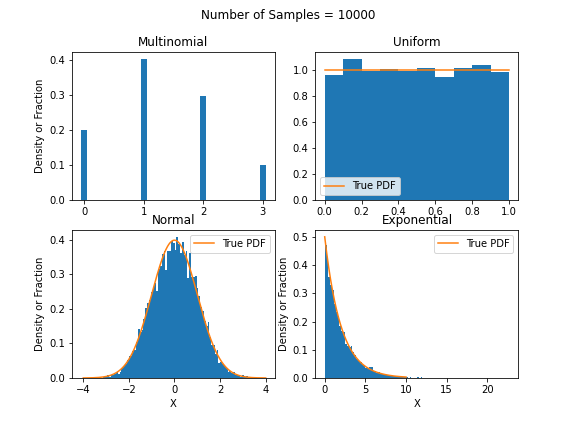
\includegraphics[width=10cm]{Q1_10000.png}
            \end{center}
            \caption{Histogram obtained after sampling $N=10000$ samples.}
        \end{figure}
        We observe that as we increase the number of samples the plotted histogram and the true PDF tend to match. This way we are 
        guaranteed that the samples were drawn from the same distribution. 

    \item \textbf{Solution 1:}
    Using Central Limit Theorem, we know that if $X_{1}, X_{2}, ..., X_{n}$ are i.i.d. random variable with mean $\mu$ and variance
    $\sigma^{2}$, then 
    \begin{equation}
    \nonumber
        \sqrt(n) \frac{\bar{X_{n}} - \mu}{\sigma} \xrightarrow[]{n \rightarrow \infty} \mathcal{N}(0, 1)
    \end{equation}
    where $\bar{X_{n}}$ is the sample mean. Now, we have samples from uniform distribution between 0 and 1 i.e., $\mu=1/2$ and $\sigma^{2}=1/12$.
    The sample mean of these samples will be a sample from standard normal distribution. We can generate samples from a normal distribution
    with mean $\mu$ and $\sigma$, using the transformation $y = \sigma z + \mu$, where z is the sample from standard normal distribution.\par
	
	\noindent %The next paragraph is not indented
    The following histogram plots the samples drawn from normal distribution with $\mu=2$ and $\sigma=2$ using the method described above. 
    The graph also shows the true PDF for the normal distribution. Since, the two match, we are guaranteed that the samples were drawn from the
    normal distribution with $\mu=2$ and $\sigma=2$.
    \par
	
	\noindent %The next paragraph is not indented
    \begin{figure}[H]
        \begin{center}
        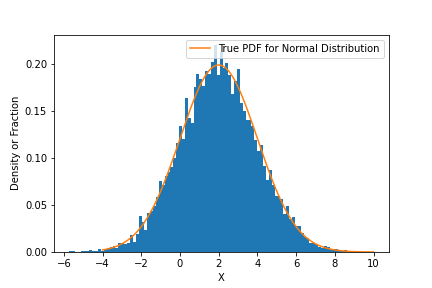
\includegraphics[width=8cm]{Q2_1.png}
        \end{center}
        \caption{Histogram obtained after sampling $N=10000$ samples.}
    \end{figure} 
    \textbf{Solution 2:}
    Let $U \stackrel{}{\sim} Unif(0, 1)$ and $\Phi(x)$ denote the standard normal CDF. Then, we can show that if $X = \Phi^{-1}(U)$,
    then $X \stackrel{}{\sim} \mathcal{N}(0, 1)$. This is because $P(X \le t) = P(\Phi^{-1}(U) \le t) = P(U \le \Phi(t)) = \Phi(t)$. Now,
    since the CDF X is $\Phi(x)$, hence, $X \stackrel{}{\sim} \mathcal{N}(0, 1)$. \par
	
	\noindent %The next paragraph is not indented
    Let $u$ be a sample from $Unif(0, 1)$. Then using the above fact, we can generate samples from standard normal random samples as 
    $x =\Phi^{-1}(u)$. Then, to generate normal samples with mean $\mu$ and variance $\sigma^{2}$ we can simply transform as 
    $y = \sigma x + \mu$, where $y$ is the sample from normal random variable with mean $\mu$ and variance $\sigma^{2}$.\par
	
	\noindent %The next paragraph is not indented
    The plotted histogram are the samples drawn using the method described above using $\mu=1$ and $\sigma^{2}=1$. The graph also shows
    the true PDF for the standard normal distribution. Since, the two match, we are guaranteed that the samples were drawn from the
    standard normal distribution.

    \begin{figure}[H]
        \begin{center}
        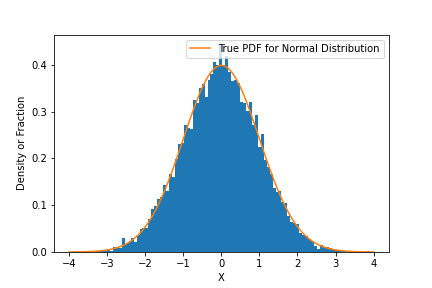
\includegraphics[width=8cm]{Q2.png}
        \end{center}
        \caption{Histogram obtained after sampling $N=10000$ samples.}
    \end{figure}

    \par
	
	\noindent %The next paragraph is not indented

    \item In order to compute the integral, we can represent the integration as an expectation of a random 
    variable. Then using Law of Large Numbers, we can compute the expectation, by sampling from the distribution of that random variable.\par
	
	\noindent %The next paragraph is not indented
    Let's $X \stackrel{}{\sim} Unif(0, \pi)$ and $f(x)$ be it's PDF i.e.,
    \begin{equation}
    \nonumber
    f(x) = \begin{cases}
        \frac{1}{\pi} & if 0 \le x \le \pi \\
        0 & otherwise
    \end{cases}
    \end{equation} 
        \begin{enumerate}
            \item The graph for $\sqrt(sin(x))$ is plotted as below:
                \begin{figure}[H]
                    \begin{center}
                    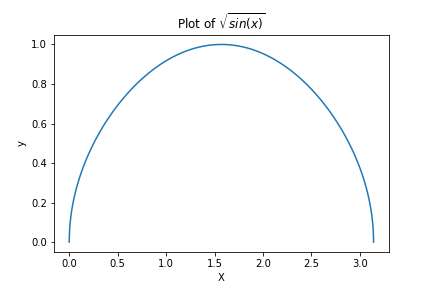
\includegraphics[width=8cm]{Q3_1.png}
                    \end{center}
                    \caption{Graph for $\sqrt(sin(x))$}
                \end{figure}
                Let $g(X) = \sqrt(sin(X))$, where $X$ is as defined above. Then 
                \begin{equation}
                    \mathbb{E}[g(X)] = \int_{-\infty}^{\infty}g(x)f(x) \,dx =  \frac{1}{\pi}\int_{0}^{\pi}g(x) \,dx
                \end{equation}
                Let $X_{1}, X_{2}, ..., X_{N} \stackrel{i.i.d.}{\sim}$ Unif$(0, \pi)$ and $Y_{i} = g(X_{i})$ for $i \in {1, 2, ... N}$. 
                Then according to Law of Large Numbers, we have 
                \begin{equation}
                    \nonumber
                    \lim_{N\to\infty} \frac{1}{N}\sum_{i=1}^{N}Y_{i} = \mathbb{E}[g(X)]
                \end{equation}
                Therefore,
                \begin{equation}
                    \int_{0}^{\pi}\sqrt(sin(x)) \,dx =  \pi \left ( \lim_{N\to\infty} \frac{1}{N}\sum_{i=1}^{N}Y_{i} \right )
                \end{equation}
                The value of the integral obtained by this method is $2.4061907079036167$.

            \item The graph for $\sqrt(sin(x))exp(-x^{2})$ is plotted as below:
            \begin{figure}[H]
                \begin{center}
                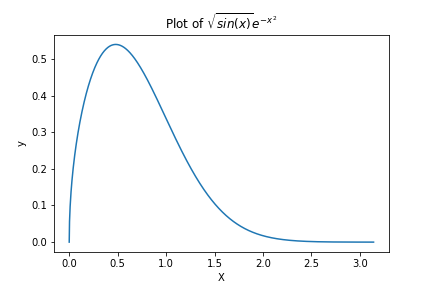
\includegraphics[width=8cm]{Q3_2.png}
                \end{center}
                \caption{Graph for $\sqrt(sin(x))exp(-x^{2})$}
            \end{figure}

			\textbf{Using Normal Random Variable}\par
	
			\noindent %The next paragraph is not indented 
			Let $X \stackrel{}{\sim} \mathcal{N} (0, \frac{1}{2})$ where $\frac{1}{2}$ is the variance $X$. Now, to apply the above trick of converting integral into
			expectation of a random variable, we need to confine the density of the above random variable between $[0, \pi]$. To do this we construct a new random 
			variable Y such that we sample from the distribution of $|X|$ and discard the samples which are greater than $\pi$. Once, we do this we can write the
			integral as:
			\begin{equation}
			\nonumber
				\int_{0}^{\pi}\sqrt(sin(x))exp(-x^2) \,dx = \lambda \left ( \lim_{N\to\infty} \frac{1}{N}\sum_{i=1}^{N}\sqrt(sin(Y_{i})) \right )
			\end{equation}
			where $Y_{i} \stackrel{i.i.d.}{\sim} Y$ 
            Now, all that remains is to determine the value of $\lambda$. This can be determined if we compute the PDF for $Y$. We know that the PDF of $|X|$ is 
			defined as follows:
			\begin{equation}
			\nonumber
				f_{x}(|X|) = \frac{2\sqrt{2}}{\pi} exp(-x^2)
			\end{equation}
			We know that the PDF of $Y$ is:
			\begin{equation}
			\nonumber
				f_{y}(Y) = \begin{cases}
				 Cf_{x}(|X|) & if 0 \le X \le \pi \\
				0 & otherwise
				\end{cases}
			\end{equation}
			where $C$ is a normalizing constant such that
			\begin{equation}
			\nonumber
				\begin{gathered}
				\int_{0}^{\pi} f_{y}(Y) \,dy = 1 \\
				\implies \int_{0}^{\pi} Cf_{x}(|X|) \,dx = 1 \\
				\implies C = \frac{1}{\int_{0}^{\pi} f_{x}(|X|) \,dx}
				\end{gathered}
			\end{equation}
			We can numerically estimate the value of $\int_{0}^{\pi} Cf_{x}(|X|) \,dx$ by using samples from Uniform distribution and applying the procedure as in part(a). 
			We found this value to be 0.7956. Therefore, $C = 1.2569$. Therefore, 
			\begin{equation}
			\nonumber
				\lambda = \frac{2\sqrt{2}C}{\pi}
			\end{equation}
			
			Using, the technique above we found the value of integral $\int_{0}^{\pi}\sqrt(sin(x))exp(-x^2) \,dx$ to be 0.570899 with just 10 samples from $Y$.
			
			\textbf{Using Uniform Random Variable}\par
	
			\noindent %The next paragraph is not indented 
            We can follow the same procedure as in part (a) but by defining $g(X) = \sqrt(sin(X))exp(-X^{2})$. The value of the integral
            obtained by this method is $0.501713$ with 10 samples from the uniform distribution. \\
			Clearly, we can see the value obtained from uniform distribution is way far-off from the value obtained from normal distribution. Therefore, we can say 
			that using Normal Distribution is sample-efficient.
        \end{enumerate}
        \par \par
	
	    \noindent %The next paragraph is not indented 

    \item
        \textbf{Assumption:} If the die shows up 2 when in the state 7, the player remains in the same state.
        The Markov Chain for the game can be drawn as follows:\par
	
	    \noindent %The next paragraph is not indented 
        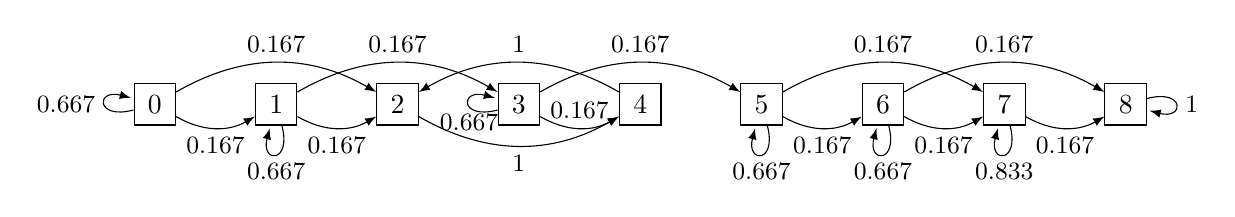
\begin{tikzpicture}[
            mynode/.style={
            draw,
            minimum size=1.5em
            },
            every loop/.append style={-latex},  
            start chain=going right  
            ]
            \foreach \Value in {0,...,8}
            \node[mynode,on chain] (s\Value) {${\Value}$};
            \path[-latex]
            (s0) edge[bend right] node[auto,swap,font=\small] {$0.167$} (s1)
            (s0) edge[bend left] node[above,swap,font=\small] {$0.167$} (s2)
            (s1) edge[bend right] node[auto,swap,font=\small] {$0.167$} (s2)
            (s1) edge[bend left] node[above,swap,font=\small] {$0.167$} (s3)
            (s2) edge[bend right] node[auto,swap,font=\small] {$1$} (s4)
            (s3) edge[bend right] node[above,swap,font=\small] {$0.167$} (s4)
            (s3) edge[bend left] node[above,swap,font=\small] {$0.167$} (s5)
            (s4) edge[bend right] node[auto,swap,font=\small] {$1$} (s2)
            (s5) edge[bend right] node[auto,swap,font=\small] {$0.167$} (s6)
            (s5) edge[bend left] node[above,swap,font=\small] {$0.167$} (s7)
            (s6) edge[bend right] node[auto,swap,font=\small] {$0.167$} (s7)
            (s6) edge[bend left] node[above,swap,font=\small] {$0.167$} (s8)
            (s7) edge[bend right] node[auto,swap,font=\small] {$0.167$} (s8)
            (s0) edge[loop left] node[left,font=\small] {$0.667$} (s0)
            (s1) edge[loop below] node[below,font=\small] {$0.667$} (s1)
            (s3) edge[loop left] node[below,font=\small] {$0.667$} (s3)
            (s5) edge[loop below] node[below,font=\small] {$0.667$} (s5)
            (s6) edge[loop below] node[below,font=\small] {$0.667$} (s6)
            (s7) edge[loop below] node[below,font=\small] {$0.833$} (s7)
            (s8) edge[loop right] node[right,font=\small] {$1$} (s8);
        \end{tikzpicture}

        The transition probability matrix can be represented as follows:
        \begin{equation}
        \nonumber
            Q = \begin{bmatrix}
                2/3 & 1/6 & 1/6 & 0 & 0 & 0 & 0 & 0 & 0 \\
                0 & 2/3 & 1/6 & 1/6 & 0 & 0 & 0 & 0 & 0 \\
                0 & 0 & 0 & 0 & 1 & 0 & 0 & 0 & 0 \\
                0 & 0 & 0 & 2/3 & 1/6 & 1/6 & 0 & 0 & 0 \\
                0 & 0 & 1 & 0 & 0 & 0 & 0 & 0 & 0 \\ 
                0 & 0 & 0 & 0 & 0 & 2/3 & 1/6 & 1/6 & 0 \\
                0 & 0 & 0 & 0 & 0 & 0 & 2/3 & 1/6 & 1/6 \\
                0 & 0 & 0 & 0 & 0 & 0 & 0 & 5/6 & 1/6 \\
                0 & 0 & 0 & 0 & 0 & 0 & 0 & 0 & 1
                \end{bmatrix}
        \end{equation}

        The initial distribution of states can be represented as follows:
        \begin{equation}
        \nonumber
            \pi_{0} = \begin{bmatrix}
                       1 & 0 & 0 & 0 & 0 & 0 & 0 & 0 & 0
                      \end{bmatrix}
        \end{equation}

        \textbf{Simulation} \par
	
	    \noindent %The next paragraph is not indented
        We can consider an indicator random variable I such that it takes value of $1$ when the player reaches the end state else it
        takes the value of $0$. Now, the expectation of this random variable is the probability of the player ever reaching the end state.
        Using, Law of Large Numbers we can calculate this probability by simulating this Markov Chain (i.e. playing this game) multiple
        times and calculating the average number of times the player reaches the end state.\par
	
	    \noindent %The next paragraph is not indented
        The question now that arises is that how long should we simulate each game? For this we calculate the value of $\pi_{0}Q^{T}$ for
        large values of T. We observe that the values of $\pi_{0}Q^{T}$ for large values of $T$ alternate between $\begin{bmatrix} 0 & 0 & 0.482 & 0 & 0.393 & 0 & 0 &
        0 & 0.125 \end{bmatrix}$ and \\ $\begin{bmatrix} 0 & 0 & 0.393 & 0 & 0.482 & 0 & 0 & 0 & 0.125 \end{bmatrix}$. We know 
        from this that in the long run following things happen:
        \begin{itemize}
            \item The probability of player being in states 0, 1, 3, 5, 6 and 7 is almost 0.
            \item The probability of player being in states 2 and 4 alternates between 0.393 and 0.482.
            \item The probability of player being in state 8 is 0.125.
        \end{itemize}
        In other words, in the long run the player can only be in states 2, 4 or 8. Therefore, while simulating the Chain, we need to 
        only simulate to the point where the player either reaches the state 2 or 4 (then the player cannot reach end state) or the 
        point where the player reaches the state 5 (because then the player is guaranteed in the long run will reach the end state). \par
	
	    \noindent %The next paragraph is not indented
        On simulating the Chain for 10,000 times the probability of ever reaching the end state is found to be $0.12555$.

        \textbf{Analytic Solution} \par
	
	    \noindent %The next paragraph is not indented
		Let $\alpha_{i}$ denote the probability of ever-reaching the end state from state $i$. We can create the 
		following equations recursively:
		\begin{equation}
		\nonumber
		\begin{gathered}
			\alpha_{0} = \frac{1}{6} \alpha_{1} + \frac{1}{6} \alpha_{2} + \frac{2}{3} \alpha_{0} \\
			\alpha_{1} = \frac{1}{6} \alpha_{2} + \frac{1}{6} \alpha_{3} + \frac{2}{3} \alpha_{1} \\
			\alpha_{2} = \frac{1}{6} \alpha_{3} + \frac{1}{6} \alpha_{4} + \frac{2}{3} \alpha_{2} \\
			\alpha_{3} = \frac{1}{6} \alpha_{4} + \frac{1}{6} \alpha_{5} + \frac{2}{3} \alpha_{3} \\
			\alpha_{4} = \frac{1}{6} \alpha_{5} + \frac{1}{6} \alpha_{6} + \frac{2}{3} \alpha_{4} \\
			\alpha_{5} = \frac{1}{6} \alpha_{6} + \frac{1}{6} \alpha_{7} + \frac{2}{3} \alpha_{5} \\
			\alpha_{6} = \frac{1}{6} \alpha_{7} + \frac{1}{6} \alpha_{8} + \frac{2}{3} \alpha_{6} \\
			\alpha_{7} = \frac{1}{6} \alpha_{8} + \frac{5}{6} \alpha_{7} \\
		\end{gathered}
		\end{equation}
		We know that $\alpha_{2} = \alpha_{4} = 0$ and $\alpha_{8}=1$. On solving the above set of equations we get $\alpha_{5} = \alpha_{6} = \alpha_{7} = 1$, 
		$\alpha_{3} = 1/2$, $\alpha_{1} = 1/4$ and $\alpha_{0} = 1/8$. Hence, the required probability is $\alpha_{0} = 0.125$. \par
	
	    \noindent %The next paragraph is not indented
		\textbf{Another Solution} \par
	
	    \noindent %The next paragraph is not indented
        Let us consider a random variable $X_{n}$ denoting the state of the player at timestamp $n$. Let $I$ be an indicator random 
        variable such that it takes value of $1$ when the player reaches the end state else it takes the value of $0$. Now, the 
        probability of the player ever reaching the end state is sum of probabilities of it reaching the end state at timestamp 
        $T=5, 6, .... $, where the probability of a player reaching the end state at time $T$ is probability that the player is in state
        8 at time $T$ but was not in state 8 at $T-1$ since 8 is an absorbing state. We start the sum from 5 because the earliest the player can reach the end state is 
        at timestamp 5. This can be written down as follows:
        \begin{equation}
        \nonumber
            P(I = 1) = \sum_{t=5}^{\infty} P(X_{t} = 8, X_{t-1} \neq 8) = \sum_{t=5}^{\infty} P\left (X_{t} = 8, \bigcup_{i=0}^{7} (X_{t-1} = i) \right )
        \end{equation}
        The last equality holds because if the player is not in state 8 at time $T-1$ implies that the player was in one of the states 
        from $0$ to $7$. We can 
        further simplify the above equation as
        \begin{equation}
        \nonumber
        \begin{gathered}
            P(I = 1) = \sum_{t=5}^{\infty} \sum_{i=0}^{7} P(X_{t} = 8, X_{t-1} = i)\\
                     = \sum_{t=5}^{\infty} \sum_{i=0}^{7} P(X_{t} = 8 | X_{t-1} = i)P(X_{t-1} = i) \\
                     = \sum_{t=5}^{\infty} (P(X_{t} = 8 | X_{t-1} = 6)P(X_{t-1} = 6) +  P(X_{t} = 8 | X_{t-1} = 7)P(X_{t-1} = 7))\\
        \end{gathered}
        \end{equation}
        The last equality holds because the transition probabilities $P(X_{t} = 8 | X_{t-1} = i) = 0 \forall i \in {0,1,...,5}$. Now, we
        know that $P(X_{t-1} = j) = (\pi_{0}Q^{t-1})_{j}$, where $(\cdot)_{j}$ represents the jth element of the matrix. Using this we can
        simplify the above equation as
        \begin{equation}
        \nonumber
            P(I=1) = \sum_{t=5}^{\infty} \frac{1}{6}((\pi_{0}Q^{t-1})_{6}) + \frac{1}{6}((\pi_{0}Q^{t-1})_{7})
        \end{equation}
        Now, we know that $\sum_{t=0}^{\infty} A^{t}$ for any matrix $A$ converges only when the largest eigenvalue of $A < 1$. However,
        we find that the largest eigenvalue of Q is 1. So, in compute the above sum approximately, we compute it till timestamp $t=10000$ i.e.,
        \begin{equation}
        \nonumber
            P(I=1) \approx \sum_{t=5}^{10000} \frac{1}{6}((\pi_{0}Q^{t-1})_{6}) + \frac{1}{6}((\pi_{0}Q^{t-1})_{7})
        \end{equation}
        The probability thus obtained is $0.1249$, which conforms to the probability found earlier using simulation. 
\end{enumerate}
\end{document}